% Reporte del análisis de los regímenes de etiquetas. Mismo formato que docs/reporte_modelo.
% Compilar desde docs/reporte_regimenes (dos veces, para las referencias cruzadas):
%   xelatex -interaction=nonstopmode main.tex && xelatex -interaction=nonstopmode main.tex
% Las figuras y las cifras salen de scripts/figuras.py (ver el encabezado de ese archivo).
\documentclass[conference,letterpaper]{IEEEtran}
\usepackage{fontspec}
\setmainfont{TeX Gyre Termes}
\usepackage{polyglossia}
\setdefaultlanguage{spanish}
\usepackage{amsmath,amssymb}
\usepackage{graphicx}
\usepackage{booktabs}
\usepackage{array}
\usepackage{xcolor}
\usepackage{tikz}
\usetikzlibrary{positioning,arrows.meta}
\usepackage{hyperref}
\hypersetup{colorlinks=true,linkcolor=black,citecolor=black,urlcolor=blue!50!black}
\graphicspath{{figuras/}}

\newcommand{\code}[1]{\texttt{#1}}
\newcommand{\si}{\textcolor{green!45!black}{sí}}
\newcommand{\no}{\textcolor{red!70!black}{no}}

% ---------------------------------------------------------------- datos de la portada
\newcommand{\universidad}{Benemérita Universidad Autónoma de Puebla}
\newcommand{\facultad}{Facultad de Ciencias de la Computación}
\newcommand{\carrera}{Reto AgroCebada FIRA 2026}
\newcommand{\materia}{Reporte de análisis de las etiquetas}
\newcommand{\integranteA}{José Alán Pomares Valdés}
\newcommand{\integranteB}{Luis Emmanuel Ramiro Luna}
\newcommand{\integranteC}{Vicente Josimar López Martinez}
\newcommand{\correo}{pv202351433@alm.buap.mx}
\newcommand{\asesor}{Ivan Olmos Pineda}
\newcommand{\fecha}{9 de octubre de 2026}

\newcommand{\logo}[2]{%
  \IfFileExists{figuras/#1}{\includegraphics[height=2.4cm]{#1}}%
  {\fbox{\parbox[c][2.2cm][c]{2.2cm}{\centering\footnotesize\textcolor{gray}{#2}}}}}

\begin{document}

% ---------------------------------------------------------------- portada
\begin{titlepage}
  \centering
  \begin{tabular}{@{}m{2.6cm}@{}m{\dimexpr\textwidth-5.2cm}@{}m{2.6cm}@{}}
    \logo{logo_buap.png}{Logo BUAP} &
    \centering{\Large\bfseries \universidad}\\[4pt]{\large \facultad} &
    \hfill\logo{logo_fcc.png}{Logo FCC}
  \end{tabular}\par
  \vspace{4pt}\rule{\textwidth}{1.2pt}\par
  \vspace{1.2cm}
  {\large \carrera}\par\vspace{4pt}
  {\large \materia}\par
  \vspace{3cm}
  {\Huge\bfseries ¿Qué separa a los dos\\[6pt] regímenes de rendimiento?}\par
  \vspace{0.8cm}
  {\Large Descarte de causas ambientales y contraste\\[4pt] con las cifras oficiales del SIAP}\par
  \vfill
  \begin{tabular}{@{}r@{\hspace{1em}}l@{}}
    \textbf{Integrantes} & \integranteA \\
                         & \integranteB \\
                         & \integranteC \\[4pt]
    \textbf{Asesor}      & \asesor \\[4pt]
    \textbf{Contacto}    & \href{mailto:\correo}{\correo} \\
  \end{tabular}\par
  \vspace{1.5cm}
  {\large Puebla, Pue., \fecha}\par
\end{titlepage}

\noindent\textbf{\textit{Resumen.}} \bfseries Las etiquetas del reto se dividen por municipio en dos regímenes. En el
A, los rendimientos tienen dos decimales y promedian 4.49\,t/ha; en el B, están redondeados y promedian 3.05\,t/ha.
Para que el modelo sirviera en zonas sin parcelas buscamos una variable del lugar que explicara esa brecha de
1.44\,t/ha. Probamos el clima, la altitud, la fenología observada por satélite, el suelo de INEGI y la distancia al
Popocatépetl, y ninguna la explica: dentro de cada régimen no cambian el rendimiento, y parcelas vecinas con el mismo
suelo y el mismo clima difieren 1.5\,t/ha si su municipio es de distinto régimen. Las cifras oficiales del SIAP de
2023 a 2025 tampoco muestran la brecha: los municipios de ambos regímenes promedian 2.5\,t/ha. Concluimos que la
diferencia está ligada a cómo se obtuvo la etiqueta en cada municipio, ya sea por la forma de medir o por el grupo de
productores muestreado, y no a una característica de la zona.\par\mdseries

\smallskip
\noindent\textbf{\textit{Palabras clave.}} \bfseries régimen de etiquetas, generalización espacial, cebada de temporal,
SIAP, edafología, fenología.\par\mdseries

\section{Introducción}\label{sec:intro}

El modelo de la entrega predice el rendimiento de cebada con dos datos de cada parcela: el régimen de su etiqueta y
el rendimiento de sus vecinas del mismo régimen. Funciona para las 59 parcelas del reto porque están intercaladas con
las de entrenamiento, pero no responde la pregunta que más le serviría a FIRA: \emph{si se siembra una parcela en un
lugar sin parcelas medidas, ¿qué rendimiento se puede esperar?} Para eso hace falta una variable del lugar (clima,
suelo o terreno) que exista en cualquier punto del mapa.

El régimen es la pista natural. Si los cuatro municipios del régimen A rinden 1.44\,t/ha más que los cinco del B,
algo debería estar más presente en unos que en otros. Este reporte busca ese algo. Cada hipótesis de lugar se somete
a las mismas pruebas, y la Fig.~\ref{fig:embudo} resume el recorrido. Primero medimos si el ambiente generaliza a
municipios nuevos (Sección~\ref{sec:generalizacion}). Después descartamos una por una las causas de lugar
(Sección~\ref{sec:descarte}) y contrastamos el dataset con las cifras oficiales (Sección~\ref{sec:siap}). Al final
separamos lo que podemos afirmar de lo que no (Sección~\ref{sec:discusion}).

\begin{figure*}[t]
\centering
\begin{tikzpicture}[node distance=0.32cm, every node/.style={font=\footnotesize, align=center},
  caja/.style={draw=black!60, rounded corners=2pt, minimum height=1.25cm, text width=2.05cm, fill=black!3},
  fuera/.style={caja, draw=red!50!black, fill=red!5},
  queda/.style={caja, draw=blue!60!black, fill=blue!6, text width=2.5cm},
  flecha/.style={-{Stealth[length=2mm]}, black!60}]
\node[caja] (p) {Brecha A--B\\de 1.44\,t/ha\\¿causa del lugar?};
\node[fuera, right=of p] (c) {Clima y\\altitud\\Sec.~\ref{sec:clima}};
\node[fuera, right=of c] (f) {Fenología\\y verdor\\Sec.~\ref{sec:fenologia}};
\node[fuera, right=of f] (s) {Suelo\\(INEGI)\\Sec.~\ref{sec:suelo}};
\node[fuera, right=of s] (v) {Ceniza del\\Popocatépetl\\Sec.~\ref{sec:volcan}};
\node[fuera, right=of v] (o) {Nivel oficial\\del municipio\\Sec.~\ref{sec:siap}};
\node[queda, right=of o] (q) {Forma de obtener\\la etiqueta en\\cada municipio};
\draw[flecha] (p) -- (c); \draw[flecha] (c) -- (f); \draw[flecha] (f) -- (s); \draw[flecha] (s) -- (v);
\draw[flecha] (v) -- (o); \draw[flecha] (o) -- (q);
\end{tikzpicture}
\caption{Recorrido del análisis. En rojo, las causas de lugar que probamos y descartamos. En azul, la explicación que
queda en pie.}
\label{fig:embudo}
\end{figure*}

\section{Datos y criterio de descarte}\label{sec:datos}

Usamos las 138 parcelas de entrenamiento y sus 91 variables de satélite, clima y topografía, las mismas del modelo.
Agregamos tres fuentes externas (carpeta \code{data/externos}). La primera es la carta edafológica 1:250\,000 de
INEGI, hoja E14-2, en sus Series I y II, que cubre las 197 parcelas~\cite{inegi_eda}. La segunda es el cierre agrícola
municipal del SIAP de 2023 a 2025, para cebada grano de temporal en primavera-verano~\cite{siap}. La tercera es la
literatura técnica y los reportes de caída de ceniza de 2025.

Una variable del lugar que cause la brecha debe pasar tres pruebas:
\begin{enumerate}
\item \textbf{Diferir entre regímenes} en la dirección correcta.
\item \textbf{Explicar el rendimiento dentro de cada régimen.} Si una variable baja el rendimiento 1.4\,t/ha entre
regímenes, también debe bajarlo, en proporción, entre parcelas del mismo régimen.
\item \textbf{Sostenerse entre vecinos.} Dos parcelas cercanas, con el mismo valor de la variable y de distinto
régimen, deberían rendir parecido.
\end{enumerate}
La tercera prueba es la más fuerte, porque el régimen y la geografía están casi confundidos: hay solo nueve
municipios. Por suerte, Singuilucan (régimen B) está en el norte, a 9\,km de Cuautepec (régimen A), y no en el sur
con los demás municipios B (Fig.~\ref{fig:mapa}). Esa frontera funciona como un experimento natural.

\begin{figure}[t]
\centering
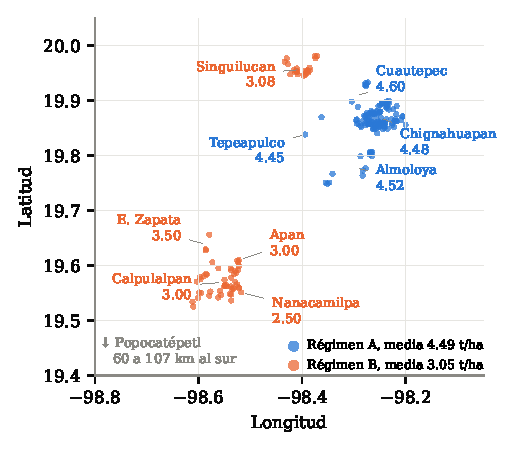
\includegraphics[width=\columnwidth]{r2_mapa}
\caption{Las 197 parcelas por régimen, con el rendimiento medio de entrenamiento de cada municipio. Singuilucan, de
régimen B, colinda con Cuautepec y Tepeapulco, de régimen A.}
\label{fig:mapa}
\end{figure}

\section{¿El ambiente generaliza a municipios nuevos?}\label{sec:generalizacion}

Para imitar la pregunta de FIRA dejamos fuera del ajuste un municipio completo, lo predijimos solo con variables de
ambiente y repetimos con los nueve municipios. Es una validación por grupos, que mide cómo se comporta un modelo
lejos de sus datos de entrenamiento~\cite{roberts2017}. Usamos ridge y un bosque aleatorio poco profundo, y
reportamos el mejor de los dos (Fig.~\ref{fig:lomo}).

\begin{figure}[t]
\centering
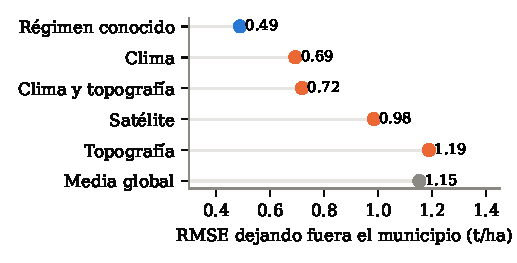
\includegraphics[width=\columnwidth]{r1_generalizacion}
\caption{Error al predecir un municipio que no se vio en el ajuste. El régimen conocido es la referencia: supone que
se sabe el régimen del municipio nuevo.}
\label{fig:lomo}
\end{figure}

El clima predice mejor que la media global (0.69 contra 1.15\,t/ha), pero muy lejos de conocer el régimen (0.49).
Además, esa capacidad no aparece dentro de los regímenes. Con el mismo esquema, aplicado a las parcelas de un solo
régimen, clima y topografía no mejoran la media: 0.536 contra 0.533\,t/ha en el A, y 0.471 contra 0.402 en el B.
Esto significa que el clima predice el nivel del municipio porque distingue la zona norte de la sur, no porque
explique el rendimiento. Con este resultado la pregunta cambia: ¿hay alguna variable del lugar detrás de la brecha?

\section{Descarte de las causas del lugar}\label{sec:descarte}

\subsection{Clima y altitud}\label{sec:clima}

Las variables que más difieren entre regímenes son climáticas (Tabla~\ref{tab:clima}). Para medir cuánto de la brecha
podrían explicar, estimamos su efecto dentro de los regímenes con una regresión que controla por régimen, y lo
multiplicamos por la diferencia entre regímenes. Ninguna explica más de 0.11 de las 1.44\,t/ha, y ningún efecto es
significativo. La altitud media casi no cambia: 2690\,m en A y 2638\,m en B.

\begin{table}[t]
\centering
\caption{Variables con mayor diferencia entre regímenes}
\label{tab:clima}
\footnotesize
\begin{tabular}{@{}lrrrr@{}}
\toprule
Variable & Dif.\ A$-$B & Efecto & $p$ & Brecha \\
 & (desv.) & (t/ha/desv.) & & (t/ha) \\
\midrule
Anomalía de lluvia en siembra & $-1.76$ & $-0.064$ & 0.42 & 0.11 \\
Lluvia en siembra & $-1.64$ & $-0.066$ & 0.34 & 0.11 \\
Amplitud térmica & $-1.64$ & $-0.053$ & 0.44 & 0.09 \\
Anomalía de Tmax, may--sep & $1.59$ & $0.049$ & 0.45 & 0.08 \\
\midrule
Brecha observada & & & & 1.44 \\
\bottomrule
\end{tabular}
\end{table}

El experimento natural de Singuilucan es más claro (Tabla~\ref{tab:zonas}). Singuilucan tiene la misma temperatura
mínima y la misma amplitud térmica que el régimen A, más lluvia y un cultivo igual de verde o más, y aun así rinde
como el B del sur. El clima no puede ser la causa.

\begin{table}[t]
\centering
\caption{Medianas por zona. B norte es Singuilucan}
\label{tab:zonas}
\footnotesize
\begin{tabular}{@{}lrrr@{}}
\toprule
 & A & B norte & B sur \\
\midrule
Rendimiento (t/ha) & 4.52 & \textbf{3.20} & 3.00 \\
Tmin may--sep (°C) & 14.0 & \textbf{14.0} & 13.0 \\
Amplitud térmica (°C) & 9.6 & 9.8 & 10.6 \\
Lluvia may--oct (mm) & 899 & \textbf{1262} & 884 \\
NDVI máximo, Planet & 0.72 & \textbf{0.79} & 0.74 \\
Verdor acumulado en el pico & 14.3 & \textbf{15.7} & 14.8 \\
Duración del verdor (días) & 152 & 119 & 133 \\
\bottomrule
\end{tabular}
\end{table}

\subsection{Fenología y verdor}\label{sec:fenologia}

La única diferencia real que encontramos en el satélite está en el calendario del cultivo. Según la serie de Planet,
el régimen A emerge alrededor del 6 de junio y el B del 16 de junio, y el verdor del A dura hasta el 6 de noviembre,
contra el 26 de octubre del B. Esto coincide con la recomendación técnica de sembrar las variedades tardías hasta el
10 de junio y las precoces en la segunda quincena de junio~\cite{inifap_hgo}. Un ciclo más largo da más tiempo de
llenado de grano, así que la hipótesis tiene sentido agronómico.

Sin embargo, no pasa la segunda prueba (Fig.~\ref{fig:fenologia}). Dentro del régimen A, las 35 parcelas que
emergieron después del 7 de junio rinden 4.47\,t/ha y las 52 tempranas, 4.50. Dentro de cada régimen, la correlación
del rendimiento con la fecha de emergencia, la duración del ciclo o el NDVI máximo está entre $-0.15$ y $0.25$.
Tepeapulco emerge tan tarde como Singuilucan y rinde 4.45 contra 3.08. El régimen A rinde alrededor de 4.5\,t/ha sin
importar cuándo se sembró.

\begin{figure}[t]
\centering
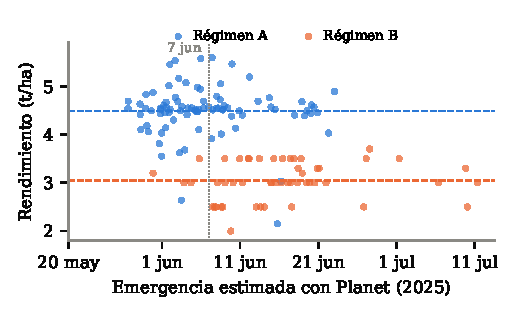
\includegraphics[width=\columnwidth]{r3_fenologia}
\caption{Rendimiento contra fecha de emergencia. Las líneas punteadas son la media de cada régimen. La siembra tardía
no baja el rendimiento del régimen A.}
\label{fig:fenologia}
\end{figure}

\subsection{Suelo}\label{sec:suelo}

El suelo era el mejor candidato restante, porque actúa parejo sobre toda una zona y no viene en los datos del reto.
La literatura señalaba el tepetate (fase dúrica) de los Llanos de Apan como limitante. Asignamos a cada parcela la
unidad de suelo que ocupa la mayor parte de su superficie en la carta de INEGI.

Si el suelo causara la brecha, se cumplirían dos cosas. Primero, dentro de un mismo régimen las parcelas con suelos
distintos rendirían distinto. Segundo, las parcelas con el mismo suelo rendirían parecido aunque fueran de distinto
régimen, y la brecha desaparecería. No se cumple ninguna (Fig.~\ref{fig:suelo}):
\begin{itemize}
\item \textbf{Distinto suelo, mismo rendimiento.} En el régimen A, los cinco grupos de suelo rinden entre 4.33 y
4.56\,t/ha. En el B, el Phaeozem y el Umbrisol rinden 3.05 y 3.02. Cambiar de suelo no mueve el rendimiento.
\item \textbf{Mismo suelo, la misma brecha.} Al comparar parcelas con el mismo suelo, la brecha entre regímenes sigue
entre 1.45 y 1.77\,t/ha, igual que la brecha total de 1.44. Hay dos unidades presentes en ambos regímenes. En el
Phaeozem con Durisol, Almoloya (A) rinde 4.63 y Calpulalpan y Emiliano Zapata (B) rinden 3.08. En el Umbrisol con
Vertisol, Cuautepec (A) rinde 4.68 y Singuilucan (B) rinde 2.91.
\item \textbf{El tepetate no está donde haría falta.} Es más común en el régimen A que en el B (53 parcelas contra
27), y en el A rinde 4.45, igual que sin tepetate.
\end{itemize}
Si el suelo fuera la causa, los puntos de la Fig.~\ref{fig:suelo} se agruparían por suelo. En cambio, se agrupan por
régimen: todo el azul cerca de 4.5 y todo el naranja cerca de 3, sea cual sea el suelo. La carta de INEGI es
1:250\,000, así que describe el suelo dominante de unidades de varios kilómetros cuadrados y no el de cada parcela.
Una diferencia de suelo más fina no se puede descartar con este mapa, pero tendría que seguir exactamente la frontera
entre municipios.

\begin{figure}[t]
\centering
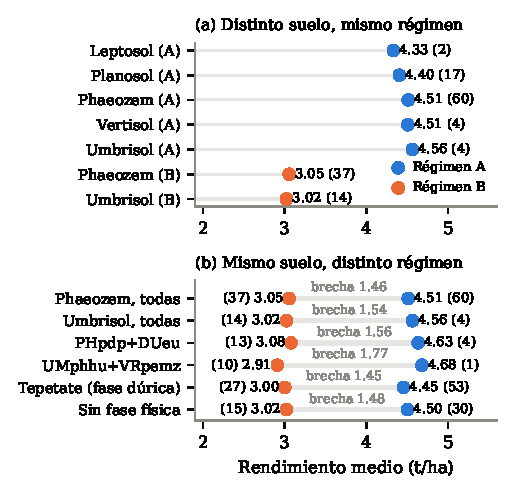
\includegraphics[width=\columnwidth]{r4_suelo}
\caption{Rendimiento medio por suelo y régimen, con el número de parcelas entre paréntesis. (a) Dentro de cada
régimen, el suelo no cambia el rendimiento. (b) Con el mismo suelo, la brecha entre regímenes sigue siendo de 1.5\,t/ha.
PHpdp+DUeu y UMphhu+VRpemz son las dos unidades que aparecen en ambos regímenes.}
\label{fig:suelo}
\end{figure}

\subsection{Ceniza del Popocatépetl}\label{sec:volcan}

Los municipios B del sur son los más cercanos al volcán (60 a 68\,km), y en enero de 2025 Cenapred reportó caída de
ceniza en Calpulalpan y Nanacamilpa~\cite{ceniza_ene25}. Tres hechos descartan esta causa. Primero, Singuilucan es el
municipio más lejano (106\,km) y rinde como B (Fig.~\ref{fig:volcan}). Además, a esa distancia una nube de ceniza mide
decenas de kilómetros de ancho y no distingue parcelas a 9\,km entre sí. Segundo, la ceniza de enero cayó antes de la
siembra, y de mayo a octubre de 2025 los pronósticos dirigían la ceniza al oeste y suroeste, lejos de la
zona~\cite{ceniza_2025}. Tercero, la ceniza daña al cultivo reduciendo su área foliar y adelantando la
senescencia~\cite{ligot2023}, pero el régimen B tiene igual o más verdor que el A.

\begin{figure}[t]
\centering
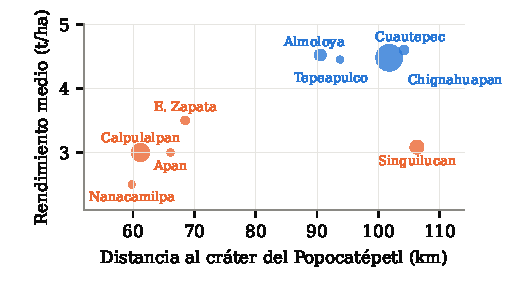
\includegraphics[width=\columnwidth]{r5_volcan}
\caption{Rendimiento medio por municipio contra la distancia al cráter. El tamaño indica el número de parcelas.}
\label{fig:volcan}
\end{figure}

\section{Contraste con las cifras oficiales}\label{sec:siap}

Si la brecha fuera una característica de la zona, aparecería también en la estadística oficial de esos municipios.
Para comprobarlo comparamos la media del reto de cada municipio con el rendimiento del cierre agrícola del SIAP de
2023, 2024 y 2025 (Fig.~\ref{fig:siap}).

\begin{figure}[t]
\centering
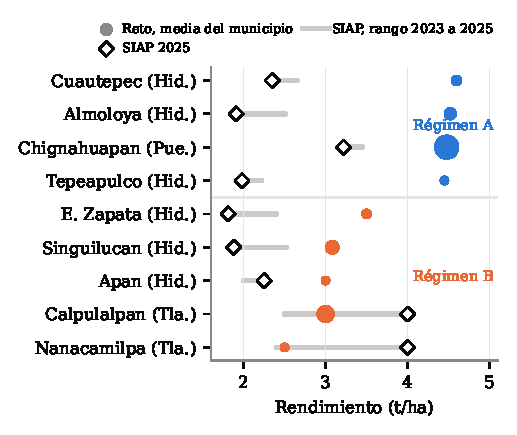
\includegraphics[width=\columnwidth]{r6_siap}
\caption{Rendimiento medio del reto por municipio (círculos, tamaño según el número de parcelas) contra el
rendimiento oficial del SIAP para cebada grano de temporal, primavera-verano.}
\label{fig:siap}
\end{figure}

\begin{itemize}
\item \textbf{En el SIAP no hay brecha entre regímenes.} El promedio de 2023 a 2025 es 2.51\,t/ha en los municipios A
y 2.48 en los B. En el reto es 4.51 contra 3.02.
\item \textbf{En Hidalgo, dentro de la misma zona, los dos regímenes rinden igual.} En 2025, Almoloya, Cuautepec y
Tepeapulco (A) tuvieron 1.91, 2.35 y 1.98\,t/ha, y Singuilucan, Apan y Emiliano Zapata (B) tuvieron 1.88, 2.25 y
1.81.
\item \textbf{En 2025, el SIAP muestra lo contrario del reto.} Calpulalpan y Nanacamilpa (B) tuvieron 4.00\,t/ha,
más que Chignahuapan (3.22). El reto les da 3.00 y 2.50 contra 4.48.
\item \textbf{Todo el régimen A queda muy por arriba de lo oficial.} Su media supera a la del SIAP 2025 de su
municipio entre 1.26 y 2.61\,t/ha. En el régimen B, la diferencia va de $-1.50$ a $+1.69$.
\item \textbf{El nivel oficial no predice las etiquetas.} La correlación entre la media del reto y la del SIAP por
municipio es $-0.43$ en 2025 y $-0.13$ en el promedio de los tres años. Usar el SIAP 2025 para predecir las parcelas
de un municipio nuevo da un RMSE de 1.47\,t/ha, peor que la media global (1.15).
\end{itemize}

El SIAP también tiene limitaciones. Es una estimación agregada de todos los productores del municipio, y en Tlaxcala
2025 trae valores redondos (4.00 y 5.00), señal de estimaciones. Aun así, es una fuente independiente que aplica el
mismo criterio a todos los municipios, y no reproduce la brecha.

\section{Discusión: qué podemos afirmar}\label{sec:discusion}

La Tabla~\ref{tab:resumen} reúne las pruebas. Ninguna causa del lugar pasa las tres, y la única explicación
compatible con todos los resultados es la forma de obtener la etiqueta en cada municipio. Esa explicación es la que
mejor encaja con el salto exacto en la frontera municipal y con el cambio de formato (dos decimales contra
redondeo).

\begin{table}[t]
\centering
\caption{Resumen de las hipótesis}
\label{tab:resumen}
\footnotesize
\begin{tabular}{@{}lccc@{}}
\toprule
Hipótesis & Difiere & Explica dentro & Se sostiene \\
 & entre A y B & del régimen & entre vecinos \\
\midrule
Clima & \si & \no & \no \\
Altitud & \no & \no & \no \\
Calendario y ciclo & \si & \no & \no \\
Suelo & \no & \no & \no \\
Ceniza volcánica & \si & \no & \no \\
Nivel oficial (SIAP) & \no & --- & \no \\
Origen de la etiqueta & \si & --- & \si \\
\bottomrule
\end{tabular}
\end{table}

\textbf{Lo que sí podemos afirmar.} La brecha de 1.44\,t/ha no se explica por el ambiente ni aparece en las cifras
oficiales. Está ligada a cómo se obtuvo el rendimiento en cada municipio, y la muestra del régimen A no representa el
nivel de su municipio.

\textbf{Lo que no podemos afirmar.} Con estos datos no se pueden separar dos causas:
\begin{itemize}
\item \emph{Sesgo de medición:} el rendimiento del régimen A se midió o se reportó de otra forma.
\item \emph{Sesgo de selección:} en los municipios A se muestrearon productores mejores que el promedio, por ejemplo
con contrato de compra, crédito o asistencia técnica, que sí obtienen alrededor de 4.5\,t/ha.
\end{itemize}
En el segundo caso sí habría una variable real, pero sería del productor y no del lugar. Tampoco podemos afirmar que
el régimen B esté sesgado. Su redondeo agrega ruido, de unas 0.14\,t/ha por parcela, pero su nivel queda cerca de lo
oficial.

\textbf{Implicaciones.} Para la calificación del reto no cambia nada: las 59 parcelas a predecir vienen de las mismas
fuentes, así que el modelo con régimen sigue siendo el adecuado. Para FIRA, el rendimiento en un lugar nuevo no se
puede estimar con el ambiente disponible, porque en estos datos el rendimiento depende más de quién siembra que de
dónde. Si el régimen A resulta ser un grupo de productores con acceso a crédito o a un esquema de contrato, ese
acceso se asociaría con casi el doble del rendimiento municipal oficial, y eso se conecta directamente con la
inclusión financiera.

\section{Conclusiones}\label{sec:conclusiones}

Buscamos una variable del lugar que explicara por qué el régimen A rinde 1.44\,t/ha más que el B, para estimar el
rendimiento en zonas sin parcelas. Con tres pruebas (diferir entre regímenes, explicar el rendimiento dentro de cada
uno y sostenerse entre vecinos) descartamos el clima, la altitud, el calendario, el suelo y la ceniza volcánica, y el
SIAP confirmó que los municipios de ambos regímenes rinden lo mismo, alrededor de 2.5\,t/ha. La brecha es una
propiedad de cómo se obtuvo la etiqueta en cada municipio, no de la zona. El modelo de la entrega sigue siendo válido
para las 59 parcelas. Para estimar en zonas nuevas harán falta datos de manejo y de productor, o rendimientos medidos
con un mismo criterio en todos los municipios.


% Sólo las referencias citadas en el texto, en estilo IEEE y en orden de aparición.
\begin{thebibliography}{10}

\bibitem{inegi_eda}
Instituto Nacional de Estadística y Geografía, ``Conjunto de datos vectorial edafológico, escala 1:250\,000, Series I
y II, hoja E14-2 Ciudad de México.'' [En línea]. Disponible: \url{https://www.inegi.org.mx/temas/edafologia/}

\bibitem{siap}
Servicio de Información Agroalimentaria y Pesquera, ``Cierre de la producción agrícola por municipio, cebada grano,
temporal, primavera-verano, 2023--2025.'' [En línea]. Disponible: \url{https://nube.agricultura.gob.mx/cierre_agricola/}.
Consultado el 9 de octubre de 2026.

\bibitem{roberts2017}
D.~R. Roberts \emph{et al.}, ``Cross-validation strategies for data with temporal, spatial, hierarchical, or
phylogenetic structure,'' \emph{Ecography}, vol.~40, no.~8, pp.~913--929, 2017.

\bibitem{inifap_hgo}
Instituto Nacional de Investigaciones Forestales, Agrícolas y Pecuarias, ``Agenda técnica agrícola de Hidalgo.''
[En línea]. Disponible:
\url{https://www.gob.mx/cms/uploads/attachment/file/1066180/Agenda_T_cnica_Agr_cola_-_Hidalgo-compressed.pdf}

\bibitem{ceniza_ene25}
``Alertan sobre caída de ceniza en varios municipios de Tlaxcala,'' \emph{Municipios Puebla}, 25 de enero de 2025.
[En línea]. Disponible:
\url{https://archivo.municipiospuebla.mx/nota/2025-01-25/tlaxcala/alertan-sobre-ca%c3%adda-de-ceniza-en-varios-municipios-de-tlaxcala}

\bibitem{ceniza_2025}
Azteca Puebla, reportes diarios de dispersión de ceniza del Popocatépetl, mayo a octubre de 2025. [En línea].
Disponible: \url{https://www.aztecapuebla.com/noticias/}

\bibitem{ligot2023}
N.~Ligot, P.~Bogaert, S.~Biass, G.~Lobet y P.~Delmelle, ``Grain size modulates volcanic ash retention on crop foliage
and potential yield loss,'' \emph{Natural Hazards and Earth System Sciences}, vol.~23, pp.~1355--1369, 2023.

\end{thebibliography}

\end{document}
